\subsection{Pishahang Results}
\todo[inline]{Pishahang Just like you did in the presentation, explain the functionalities of the top 5 dockers and why they are taking}

\subsubsection{CPU}

\begin{figure}[h]
	\centering
	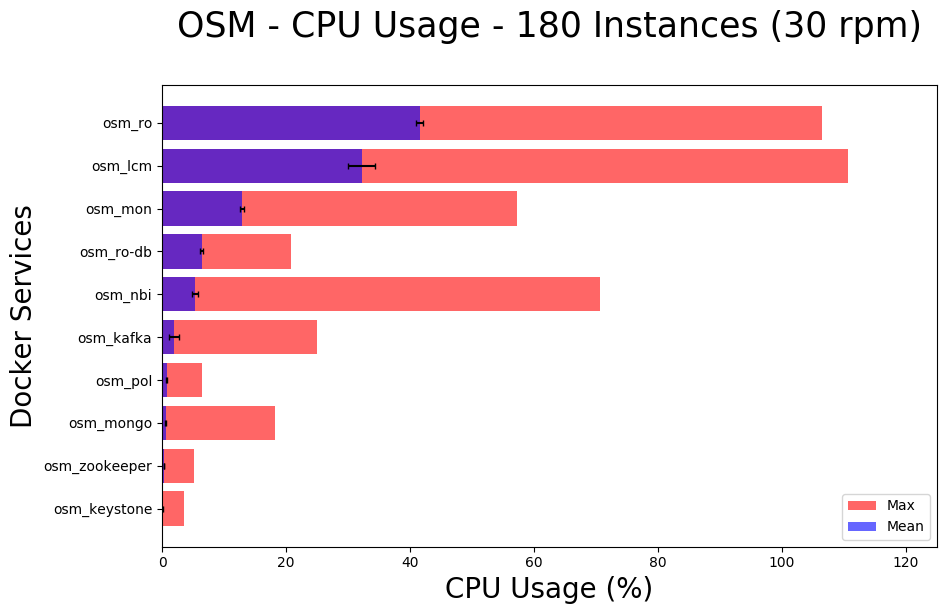
\includegraphics[width=0.7\linewidth]{../figures/scalability_graphs/Horizontal-Docker-Graphs/pishahang/cirros_case1_180-CPU}
	\caption{Pishahang CPU}
	\label{fig:cirroscase1180-cpu}
\end{figure}

\subsubsection{Memory}

\begin{figure}[h]
	\centering
	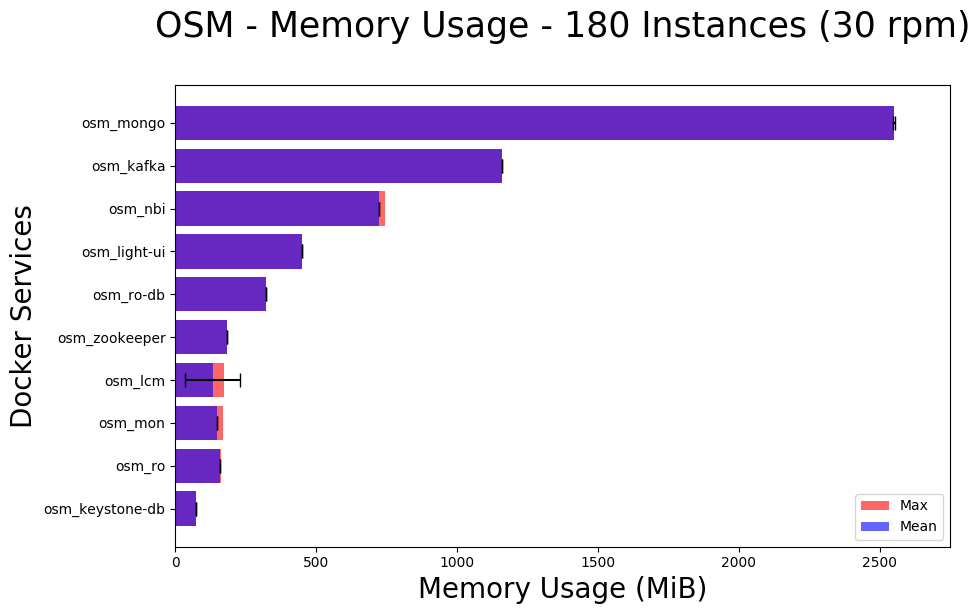
\includegraphics[width=0.7\linewidth]{../figures/scalability_graphs/Horizontal-Docker-Graphs/pishahang/cirros_case1_180-MEM}
	\caption{Pishahang MEM}
	\label{fig:cirroscase1180-mem}
\end{figure}


\subsubsection{Lifecycle}

\begin{figure}[h]
	\centering
	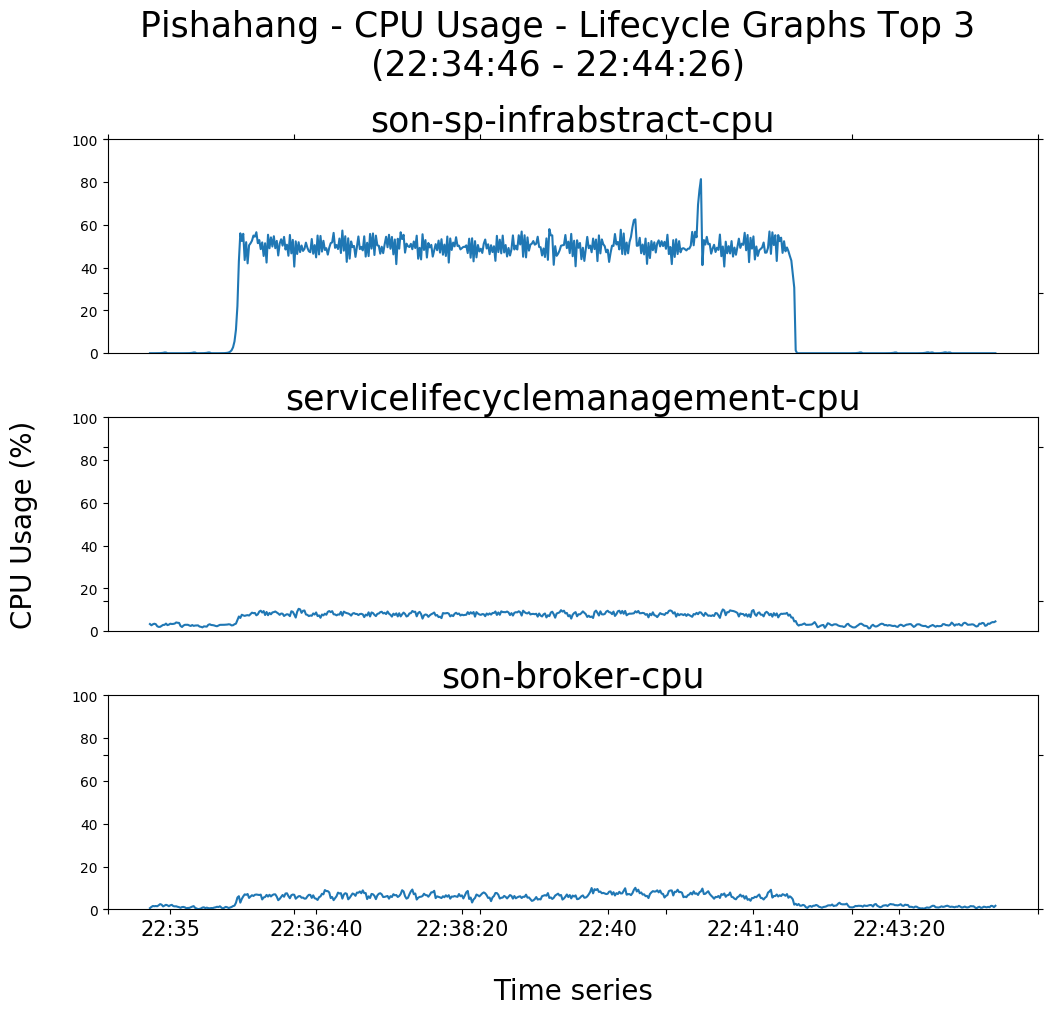
\includegraphics[width=0.7\linewidth]{figures/scalability_graphs/Lifecycle-Graphs-Top-3/Pishahang-TOP-3-Lifecycle}
	\caption{Pish LS}
	\label{fig:pishahang-top-3-lifecycle}
\end{figure}
